\documentclass[a4paper, 12pt]{article}
\usepackage[utf8]{inputenc}
\usepackage[spanish]{babel}
\usepackage{geometry}
\geometry{left=3cm, right=3cm, top=3cm, bottom=3cm}
\usepackage{graphicx}
\usepackage{hyperref}
\usepackage{titlesec}
\usepackage{fancyhdr}
\usepackage{natbib}
\bibliographystyle{plain}

% Encabezado y pie de página
\pagestyle{fancy}
\fancyhf{}
\lhead{\university}
\rhead{\faculty}
\cfoot{\thepage}
% Figura entre los nombres y la universidad

% Formato de secciones
\titleformat{\section}{\normalfont\Large\bfseries}{\thesection}{1em}{}
\titleformat{\subsection}{\normalfont\large\bfseries}{\thesubsection}{1em}{}

% Título del informe
\title{\textbf{La Automatización del Ajedrez \textit{Deep Blue}} \\ \subtitle}
\author{Daniel Machado Pérez, C411 \\ Ariel González Gómez, C412}

\newcommand{\subtitle}{\textit{Historia de la Computación}}
\newcommand{\university}{Universidad de La Habana}
\newcommand{\faculty}{Facultad de Matemática y Computación}
\newcommand{\githubrepo}{\href{https://github.com/DanielMPMatCom/Historia-de-la-Computacion.-DeepBlue.git}{Repositorio en GitHub}}

\begin{document}

% Encabezado con imágenes
\begin{figure}[t]
    
\includegraphics[width=0.15\textwidth]{assets/UH.jpg}
    \hfill
    
\includegraphics[width=0.2\textwidth]{assets/MatCom sin fondo color.png}
\end{figure}
\vspace{-2cm}

% Título principal
\maketitle

% Figura entre nombres y universidad
\begin{figure}[h!]
    \centering
    
\includegraphics[width=0.3\textwidth]{assets/logo.jpg}
\end{figure}

% Información adicional
\begin{center}
    \large \university \\
    \faculty \\
    \vspace{3.5cm}
    \githubrepo
\end{center}
\newpage
\tableofcontents
\newpage

% Resumen

\begin{abstract}
    El presente informe analiza en detalle la evolución y los 
    componentes técnicos de \textit{Deep Blue}, la primera 
    máquina capaz de derrotar al campeón mundial de ajedrez 
    bajo condiciones reglamentarias. Se describen los 
    antecedentes desde \emph{ChipTest} y \emph{Deep Thought}, la arquitectura 
    de \emph{hardware} VLSI y del clúster IBM RS/6000 SP, los 
    algoritmos de búsqueda híbrida en C con créditos diferidos y 
    la función de evaluación implementada en silicio. Además, 
    se examinan los mecanismos de paralelismo y balance de carga, 
    el soporte de libros de aperturas y bases de finales, así 
    como las estrategias de control de tiempo. Finalmente, se 
    evalúa el impacto histórico y el legado de \textit{Deep Blue} 
    en la supercomputación y la inteligencia artificial aplicada, 
    destacando su papel en el paso de enfoques de fuerza bruta a 
    sistemas híbridos con conocimiento experto.
\end{abstract}

\section*{Palabras clave}
\textit{Deep Blue}, 
ajedrez computacional, 
arquitectura paralela, 
IBM RS/6000 SP, 
búsqueda selectiva,
chip VLSI,
supercomputación.
    

\newpage
% region Introducción
% Introducción
\section{Introducción}

Desde sus inicios, el juego de ajedrez ha sido considerado un 
terreno fértil para evaluar la capacidad de las máquinas para 
replicar formas avanzadas de pensamiento humano. La complejidad 
combinatoria del ajedrez, junto con su estructura formal y 
reglas bien definidas, lo convierten en un banco de pruebas 
ideal para los sistemas de inteligencia artificial. En este 
contexto, el desarrollo de \textit{Deep Blue} por parte de IBM 
representa un hito en la historia de la computación, no solo por 
su impacto mediático, sino también por los avances técnicos y 
conceptuales que introdujo en la automatización del razonamiento 
estratégico.

\textit{Deep Blue} no fue un simple programa de ajedrez, sino un 
sistema computacional altamente especializado que integraba 
componentes de \emph{hardware} diseñados específicamente para el 
cálculo masivo de posiciones y movimientos posibles, junto con 
sofisticados algoritmos de búsqueda y evaluación posicional. La 
arquitectura del sistema combinó miles de procesadores en 
paralelo con chips dedicados a operaciones de ajedrez, 
permitiendo una profundidad de búsqueda y una velocidad de 
procesamiento inalcanzables para cualquier computadora 
convencional de su época.

Más allá de su capacidad para vencer a un campeón mundial, lo 
que convierte a \textit{Deep Blue} en un objeto de estudio 
técnico relevante es su enfoque híbrido de solución: una 
articulación precisa entre potencia de cálculo, paralelismo 
masivo y conocimiento experto codificado. Este informe se centra 
en analizar los componentes técnicos que hicieron posible dicha 
hazaña, incluyendo tanto los aspectos de \emph{hardware} como los 
mecanismos algorítmicos empleados, y cómo estos interactúan de 
forma coordinada para lograr un rendimiento sobresaliente en la 
resolución de un problema complejo como el ajedrez.

El objetivo de este estudio no es explorar los aspectos 
históricos del enfrentamiento entre \textit{Deep Blue} y Garry 
Kasparov, aunque se comentará brevemente su contexto; el foco 
principal recae sobre los elementos estructurales y funcionales 
del sistema, desde su arquitectura paralela hasta las 
heurísticas que guían la evaluación de posiciones. A través de 
este análisis técnico, se busca comprender cómo la integración 
eficaz de recursos computacionales puede acercarse, e incluso 
superar, ciertas formas de cognición humana en dominios bien 
estructurados.


\newpage
% region Desarrollo
% Desarrollo


\section{Antecedentes del ajedrez computacional}


Entre finales de la década de 1940 y principios de la de 1950, 
surgieron los primeros esfuerzos teóricos y conceptuales para 
dotar a las máquinas de la capacidad de jugar al ajedrez. En 
1949, Claude E. Shannon publicó el artículo \emph{“Programming a 
Computer for Playing Chess”}, en el que planteó por primera vez 
el uso de la técnica \footnote{Algoritmo de decisión utilizado en teoría de juegos para minimizar la posible pérdida en el peor de los casos. El algoritmo asume que el oponente juega de manera óptima para maximizar su ganancia.} 
combinada con funciones de 
evaluación heurísticas y un corte alfa-beta\footnote{Optimización del algoritmo minimax que reduce el número de nodos evaluados en el árbol de búsqueda. Mejora la eficiencia descartando ramas que no pueden influir en la decisión final.} 
rudimentario para 
reducir el espacio de búsqueda \cite{shannon1950xxii}. En este 
trabajo, Shannon (considerado el padre de la teoría de la 
información) estimó la complejidad del árbol de juego de ajedrez 
en el orden de \(10^{120}\) posiciones y sugirió métodos 
sistemáticos para explorar únicamente las ramas más prometedoras, 
estableciendo así las bases de la mayoría de los programas de 
ajedrez posteriores.

Pocos años después, en 1950-1952, Alan M. Turing y David G. 
Champernowne desarrollaron “Turochamp”, el primer programa de 
ajedrez propiamente dicho, concebido para ejecutarse en el 
ordenador ACE de la National Physical Laboratory (aunque nunca 
llegó a implementarse íntegramente en máquina y fue simulado 
paso a paso por Turing en papel) \cite{turing1953digital}. A pesar de 
su simplicidad y de que un solo movimiento requería más de media 
hora de cálculo humano, Turochamp demostró que incluso un 
algoritmo basado en reglas limitadas era capaz de jugar una 
partida reconocible, articulando con ello el paradigma de 
combinar heurísticas de posición, generación de jugadas y 
cortes selectivos, prefigurando los sistemas que conformarían la 
era moderna del ajedrez computacional.

\subsection{De \emph{ChipTest} a \emph{Deep Thought}}

En la década de los 80 se manifestaban esfuerzos tempranos en 
el diseño de una máquina capaz de jugar ajedrez a un nivel comparable
al de los grandes maestros. Fue así como en la Universidad 
Carnegie Mellon nacían los proyectos \emph{ChipTest} y \emph{Deep Thought},
precursores de \textit{Deep Blue}.


\subsection{\emph{ChipTest}}
El proyecto \emph{ChipTest} se inició en 1985 bajo la dirección de 
Feng-hsiung Hsu, Thomas 
Anantharaman y Murray Campbell, con el objetivo de explorar la 
viabilidad de un generador de movimientos de ajedrez 
implementado en VLSI (\emph{Very Large Scale Integration})\footnote{Proceso de creación de circuitos integrados (chips) mediante la combinación de millones de transistores en un solo chip. Permite una alta densidad de componentes y un bajo consumo de energía.}. 
La primera versión de 
\emph{ChipTest} estaba controlada por una estación de trabajo 
Sun-3/160\footnote{Sun-3 es una serie de \emph{computer workstations} y servidores de UNIX producida por Sun Microsystems, lanzada el 9 de septiembre de 1985.} 
y alcanzaba aproximadamente 50000 posiciones por 
segundo. En 1986, \emph{ChipTest} compitió en el North 
American Computer Chess Championship (NACCC)\footnote{Campeonato 
de ajedrez computacional que se celebró entre 1970 y 1994. 
Organizado por la \emph{Association for Computing Machinery (ACM)} y por Monty Newborn, profesor de 
Ciencia de la Computación en la Universidad McGill.}, 
donde, pese a contar con 
pruebas limitadas antes del torneo, consiguió recuperarse tras 
un inicio adverso (3 derrotas) y obtuvo un empate 
\cite{hsu1990deep}.

En agosto de 1987 se rediseñó \emph{ChipTest} y se rebautizó como 
\emph{ChipTest-M}, multiplicando por diez su velocidad de búsqueda 
hasta alrededor de 500000 posiciones por segundo, ya sobre una 
Sun-4\footnote{Aparecida por primera vez en julio de 1987, con el lanzamiento de la Sun 4/260.}. 
Esta versión se alzó con el título en el 
NACCC de 1987 con un marcador de 4-0. El éxito de 
\emph{ChipTest-M} condujo al desarrollo de \emph{Deep Thought}: la versión 
0.01 apareció en mayo de 1988 y la 0.02 en noviembre del mismo 
año, incorporando dos procesadores VLSI dedicados y elevando la 
tasa de búsqueda a casi 700000 posiciones por segundo. Con \emph{Deep Thought}, el equipo obtuvo el título en 
el World Computer Chess Championship de 1989 con un resultado 
perfecto de 5-0 \cite{newborn1988results}.

\subsection{Primeros éxitos y limitaciones}

\emph{Deep Thought} destacó en 1988 al compartir el primer puesto en el 
Software Toolworks Open de Los Ángeles\footnote{Torneo de ajedrez celebrado en 1988 en Los Ángeles, notable por su relevancia en la historia del ajedrez computacional}, 
donde venció al gran 
maestro Bent Larsen, consiguiendo una valoración de rendimiento 
de 2551 según la USCF (\emph{US Chess Federation}) y ganando 
el Fredkin Intermediate Prize \cite{hsu1990grandmaster}. 
Asimismo, ganó el ACM Computer Chess 
Championship en Orlando ese mismo año \cite{hsu1990grandmaster}. Pese a 
estos logros, la arquitectura de \emph{ChipTest} y \emph{Deep Thought} 
permanecía limitada por un grado de paralelismo moderado, 
lo que restringía la profundidad uniforme de 
búsqueda y obligaba a depender intensamente de heurísticas de 
selección y extensiones locales para obtener rendimiento 
competitivo \cite{hsu1990deep}.








\section{Origen y maduración de \textit{Deep Blue}}

A finales de 1989, parte del equipo original de \emph{ChipTest} y \emph{Deep 
Thought} (Feng-hsiung Hsu, Murray Campbell, Joe Hoane, Thomas Anantharaman, 
Andreas Nowatzyk y Mike Browne) pasó al IBM T.J. 
Watson Research Center para continuar el desarrollo de máquinas 
de ajedrez de alto rendimiento. En este nuevo entorno se 
estableció el proyecto \textit{\emph{Deep Thought} 2}, considerado el 
paso intermedio hacia lo que pronto sería conocido como 
\textit{Deep Blue} \cite{campbell2002deep}. Bajo la dirección de la 
división de investigación de IBM, el sistema heredó la 
arquitectura basada en chips VLSI especializada para generar y 
evaluar movimientos de ajedrez, al tiempo que incorporaba 
herramientas de \emph{software} más avanzadas para depuración, 
afinamiento de la función de evaluación y análisis de partidas 
\cite{campbell2002deep}.

\begin{figure}[h]
    \centering
    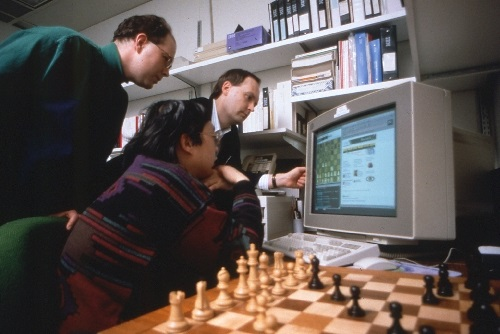
\includegraphics[width=0.6\textwidth]{assets/Deep Blue's core team, Joe Hoane, Feng-hsiung Hsu, and Murray Campbell.jpg}
    \caption{Equipo central de \textit{Deep Blue}, Joe Hoane, Feng-hsiung Hsu y Murray Campbell.}
    \label{fig:team}
\end{figure}


\subsection{\textit{Deep Blue} I (1995-1996)}

El prototipo \textit{Deep Blue I} comenzó a tomar forma en 1995, 
tras tres años de diseño de un chip de búsqueda único. La 
primera remesa de circuitos llegó en septiembre de ese año y, 
una vez solucionados los defectos iniciales, en enero de 1996 se 
dispuso de la versión estable. El sistema corría sobre un 
clúster IBM RS/6000 SP\footnote{Scalable POWERparallel es una serie discontinuada de supercomputadoras de la línea RS/6000 de IBM} 
de 36 nodos y empleaba 216 chips VLSI, 
cada uno capaz de explorar entre 1.6 y 2 millones de posiciones 
por segundo. En conjunto, la máquina alcanzaba velocidades de 
entre 50 y 100 millones de posiciones por segundo \cite{campbell2002deep}.    

En febrero de 1996, \textit{Deep Blue I} se enfrentó a Garry 
Kasparov bajo condiciones de torneo: tras empatar 2-2 en las 
cuatro primeras partidas, Kasparov ganó los dos encuentros 
finales, venciendo por 4-2 \cite{campbell2002deep}. Aunque el 
resultado favoreció al campeón humano, la serie demostró que una 
máquina especialmente diseñada podía competir de tú a tú con la 
élite mundial.

\subsection{\textit{Deep Blue} II (1996-1997)}

Tras el match de 1996 quedó patente la necesidad de mejorar la 
función de evaluación y aumentar el paralelismo. En respuesta, 
IBM diseñó un nuevo chip que amplió los rasgos de evaluación de 
alrededor de 6400 a más de 8000, incorporó detección de 
repeticiones en \emph{hardware} y optimizaciones en generación de 
jugadas, elevando la velocidad de cada chip a 2-2.5 millones de 
posiciones por segundo. Además, el sistema pasó a disponer de 
480 chips VLSI distribuidos en 30 nodos SP, duplicando con 
creces la capacidad de búsqueda \cite{campbell2002deep}.

Entre enero y mayo de 1997, el equipo dedicó la mayor parte de 
sus esfuerzos a afinar la función de evaluación y a preparar la 
base de datos de aperturas y finales\footnote{Colección exhaustiva de posiciones de ajedrez con resultados precalculados, utilizadas para acelerar la búsqueda en las fases inicial y final del juego.}. El resultado fue 
\textit{Deep Blue II}, que derrotó a Kasparov por 3\(\frac{1}{2}\)-2\(\frac{1}{2}\) en mayo
de 1997, convirtiéndose en la primera máquina en vencer al 
campeón mundial en un match reglamentario y recibiendo por 
ello el Premio Fredkin\footnote{Premio creado por Edward Frenkin para la primera computadora que venciera a un campeón mundial de ajedrez.} \cite{campbell2002deep}.



\begin{figure}[h]
    \centering
    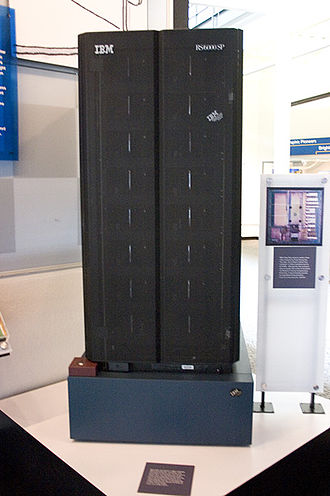
\includegraphics[width=0.6\textwidth]{assets/deepblue.jpg}
    \caption{\textit{Deep Blue}.}
    \label{fig:deepblue}
\end{figure}










\section{Arquitectura del sistema}

La solidez de la capacidad de cómputo de \textit{Deep Blue} 
descansa en su diseño arquitectónico, que combina un clúster de 
propósito general de alto rendimiento\footnote{Conjunto de computadoras interconectadas que trabajan en conjunto para resolver un problema complejo. La flexibilidad de "propósito general" permite ejecutar una variedad de tareas.} 
con cientos de 
aceleradores VLSI especializados. Esta configuración híbrida 
permite delegar las primeras fases de la búsqueda en un entorno 
distribuido de nodos IBM RS/6000 SP, optimizado para la gestión 
de tablas de transposición\footnote{Estructura de datos que almacena resultados de evaluaciones de posiciones ya analizadas, permitiendo la reutilización de información y evitando cálculos redundantes.} 
y la coordinación de tareas, y 
delegar las fases más profundas y tácticamente críticas en chips 
dedicados que ejecutan en silicio algoritmos de evaluación y 
control de búsqueda con latencia mínima \cite{campbell2002deep}. 
A continuación se presentan los principales componentes de esta 
arquitectura, desde la infraestructura de los nodos hasta la 
jerarquía maestro-trabajador-chip que maximiza el paralelismo y 
la eficiencia del sistema.

\subsection{Infraestructura IBM RS/6000 SP}

El corazón de \textit{Deep Blue} es un clúster IBM RS/6000 SP 
compuesto por treinta nodos equipados con procesadores Power2 
Super Chip (P2SC)\footnote{Microprocesadores diseñados y comercializados por IBM para servidores y supercomputadoras}, 
de los cuales veintiocho funcionan a una 
frecuencia de 120 MHz y dos a 135 MHz. Cada nodo dispone de 1 GB 
de memoria RAM y 4 GB de almacenamiento local. La interconexión 
se realiza mediante un conmutador de alta velocidad que 
implementa el estándar MPI (\emph{Message-Passing Interface Standard})\footnote{Especificación estándar para la comunicación entre nodos en un sistema de computación paralela. Define funciones y protocolos para el intercambio de mensajes.}, 
garantizando una latencia mínima en 
el envío y recepción de posiciones de ajedrez durante la 
búsqueda paralela \cite{campbell2002deep, hsu1999ibm}.

\subsection{Chips especializados}

Para alcanzar velocidades de exploración de árbol imposibles en 
un ordenador convencional, \textit{Deep Blue} emplea 480 chips 
VLSI especializados, distribuidos en los treinta nodos SP. Cada 
chip integra tres módulos fundamentales: un generador de 
movimientos basado en lógica combinatoria (matriz 8x8), una 
función de evaluación en dos niveles —rápida (un ciclo de reloj) 
y lenta (análisis columna por columna de estructuras complejas)—, 
y un controlador de búsqueda alpha-beta de ventana nula con 
extensiones locales\footnote{Variación del algoritmo alpha-beta que utiliza una ventana de búsqueda estrecha (nula) para identificar rápidamente movimientos prometedores, extendiendo la búsqueda en profundidad solo en esas ramas.} 
(jaques, peones pasados\footnote{Un \emph{peón pasado} 
es aquel que no tiene peones enemigos en su misma columna ni en 
las columnas adyacentes que puedan impedir su avance hacia la 
octava fila}, detección de 
repeticiones en 32 plies\footnote{Un \emph{ply} (o media jugada) 
corresponde al movimiento de un solo bando; dos plies equivalen 
a un movimiento completo de ambos jugadores}) \cite{campbell2002deep}. Este diseño en 
silicio permite examinar, de forma acumulada, entre 2 y 2.5 
millones de posiciones por segundo por chip. \cite{hsu1999ibm}

\begin{figure}[h!]
    \centering
    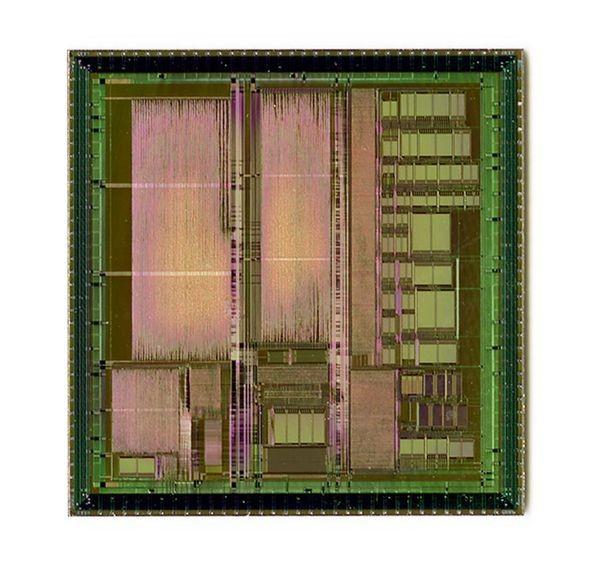
\includegraphics[width=0.6\textwidth]{assets/deep-blue-chip.jpg}
    \caption{Esquema del chip VLSI de \textit{Deep Blue}: generador de movimientos, evaluación rápida/lenta y controlador alpha-beta de ventana nula.}
    \label{fig:chip_vlsi}
\end{figure}

\subsection{Jerarquía Maestro--Trabajador--Chip}


La ejecución de la búsqueda se organiza jerárquicamente en tres 
niveles. De los procesadores SP uno es designado como maestro y el resto como trabajadores.
En el nivel superior, el nodo maestro realiza las 
primeras iteraciones de la búsqueda, explorando las ramas superiores del árbol de juego, 
generando posiciones 
“hoja” y distribuyéndolas entre los nodos trabajadores. 
A continuación, esos nodos trabajadores profundizan 
el análisis unas pocas plies más, aplicando tablas de 
transposición y heurísticas de selección. Finalmente, cada 
trabajador delega las posiciones finales a un grupo de chips 
VLSI (16 por nodo) para que realicen en \emph{hardware} la fase más 
profunda y estable de la exploración del árbol de juego. 
Esta arquitectura maestro-trabajador-chip 
maximiza el paralelismo y mantiene siempre ocupados tanto los 
procesadores como los chips especializados \cite{campbell2002deep, hsu1999ibm}.










\section{Algoritmos de búsqueda y evaluación}

La fortaleza de \textit{Deep Blue} radica en la combinación 
sinérgica de un motor de búsqueda en \emph{software} con una evaluación 
especializada en \emph{hardware}. Este enfoque híbrido permite 
explotar al máximo tanto la flexibilidad algorítmica como la 
velocidad de procesamiento en silicio.

\subsection{Búsqueda selectiva híbrida}

El motor en C emplea el algoritmo “dual credit with delayed 
extensions”, que otorga \emph{créditos} parciales a movimientos 
forzantes (FFP por sus siglas en inglés)\footnote{Secuencias de movimientos en que un 
bando efectúa una jugada forzante (como un jaque o una captura decisiva)
y el oponente está prácticamente obligado a responder de manera 
concreta} o de elevado carácter táctico  y sólo los 
\emph{canjea} cuando su acumulación supera un umbral predefinido, 
evitando así explosiones en la exploración del árbol de juego. 
Para preservar la coherencia de la 
Variación Principal\footnote{Secuencia de movimientos que el programa considera óptima para ambos bandos, según el análisis actual.}, 
cada bando mantiene su propia cuenta de 
crédito y, al extenderse uno, se descuenta el mismo importe al 
adversario, garantizando un “\emph{search envelope}”\footnote{Rango 
de profundidad mínima garantizada que el algoritmo debe mantener 
para todas las ramas relevantes, de modo que la exploración no 
oscile entre profundidades muy distintas en posiciones similares.} 
que impide 
re-búsquedas oscilantes. Gracias a este 
mecanismo, \textit{Deep Blue} ajusta dinámicamente la 
profundidad de búsqueda en función de la complejidad táctica de 
la posición, llegando a profundidades efectivas de hasta 
cuarenta plies en las variantes más forzadas \cite{campbell1999search}.

\subsection{Evaluación en \emph{hardware}}

La evaluación de posiciones se realiza completamente en 
silicio mediante más de 8000 patrones VLSI. En un primer paso, 
la evaluación rápida suma en un único ciclo de reloj los valores 
básicos de material y posicionamiento. A continuación, la 
evaluación lenta analiza columna por columna estructuras 
posicionales complejas (como seguridad de rey, configuración de 
peones y control de casillas críticas) utilizando tablas 
parametrizables cuyos pesos fueron ajustados por herramientas 
automáticas y entrenamiento comparativo. Este diseño asegura que cada 
evaluación se ejecute en tiempo constante, sin degradar la 
velocidad global de búsqueda \cite{campbell1999search}.

\subsection{Extensiones y búsqueda quiescente}

Para mitigar el “efecto horizonte”\footnote{Fenómeno que puede ocurrir 
en juegos de estrategia, especialmente en el ajedrez, donde se 
limita la capacidad de analizar las consecuencias de una jugada 
a un número finito de pasos debido a la complejidad del juego.} 
y capturar tácticas 
decisivas, \textit{Deep Blue} aplica extensiones locales y 
búsqueda quiescente\footnote{Algoritmo que se utiliza 
habitualmente para extender la búsqueda en nodos inestables en 
árboles de juego minimax en programas informáticos.} 
tanto en \emph{hardware} como en \emph{software}. 
Entre los criterios de extensión destacan la \emph{singularidad} 
(cuando un movimiento es claramente superior a todas las alternativas, 
se extiende 1-2 plies adicionales) y los \emph{jaques} o 
\emph{peones pasados}\footnote{Un \emph{peón pasado} 
es aquel que no tiene peones enemigos en su misma columna ni en 
las columnas adyacentes que puedan impedir su avance hacia la 
octava fila}, 
que reciben tratamiento 
preferente para explorar líneas forzadas. 
La detección de repeticiones se implementa mediante un buffer 
circular de 32 plies en el chip, que invalida automáticamente 
ramas cíclicas mediante un “\emph{fail-low}”\footnote{En 
las variantes de poda alfa-beta, \emph{fail-low} 
ocurre en un nodo cuando ninguna de las jugadas exploradas 
logra elevar el valor evaluado por encima de la cota inferior 
\(\alpha\). Este resultado suele emplearse 
para terminar la exploración precozmente, ahorrando cómputo en 
ramas que no pueden mejorar la decisión actual.} 
\cite{campbell1999search}.  

La búsqueda quiescente continúa hasta que no quedan capturas 
críticas ni amenazas inmediatas, garantizando que sólo se 
evalúen posiciones \emph{quietas} y evitando así que variantes 
tácticas perdidas\footnote{Situaciones en el juego donde una secuencia de movimientos forzados (táctica) lleva a una posición ventajosa que inicialmente podrían no ser evidentes y no encontrarse en el análisis.} 
distorsionen la valoración final.














\section{Paralelismo y rendimiento}

La capacidad de \textit{Deep Blue} para explorar eficientemente 
espacios de estado inmensos no habría sido posible sin un diseño 
de paralelismo multinivel cuidadosamente articulado. A lo largo 
de la búsqueda, se combinan técnicas de paralelismo en \emph{software} 
(que permiten dividir dinámicamente el árbol de juego entre 
múltiples procesadores) con un despacho asíncrono de tareas a 
cientos de chips especializados. Este enfoque mixto optimiza la 
utilización de recursos y amortigua tanto la variabilidad en los 
tamaños de las subramas como las latencias de comunicación, 
resultando en un rendimiento que, aunque superior al de cualquier 
sistema previo, revela asimismo los desafíos de la escalabilidad 
en arquitecturas de gran tamaño \cite{campbell2002deep}. 


\subsection{Paralelismo en \emph{software}}

El paralelismo en \emph{software} de \textit{Deep Blue} se articula en 
varios niveles para maximizar el aprovechamiento de los 30 
nodos SP antes de delegar en \emph{hardware}. En primer lugar, se 
emplea \emph{PV-parallelism}, donde tras explorar el primer 
movimiento de la Variación Principal (PV) todas las alternativas 
pueden evaluarse en paralelo con ventanas de búsqueda 
desplazadas para conservar la selectividad. 
En segundo lugar, en nodos de \emph{fail-high}\footnote{Un 
\emph{fail-high} se produce cuando, en la poda 
alfa-beta, la evaluación de un nodo supera la cota superior 
\(\beta\), indicando que ya existe una jugada conocida que 
anulará esa posición y, por tanto, no es necesario explorar el 
resto de sus sucesores.}, se 
pueden lanzar en paralelo búsquedas de profundidad reducida 
para refinar amenazas y extensiones, mientras que en nodos de 
\emph{fail-low} todas las ramas se procesan 
concurrentemente hasta encontrar un corte. 
Finalmente, la sincronización global se realiza al término de 
cada iteración de búsqueda, garantizando consistencia de las 
tablas de transposición y de los datos de análisis antes de 
pasar a la siguiente profundidad \cite{campbell2002deep}.

\subsection{\emph{Offloading} a \emph{hardware}}

Una vez exploradas varias capas en \emph{software}, \textit{Deep Blue} 
\emph{offloads}\footnote{En este contexto, “\emph{offload}” hace 
referencia a la transferencia asíncrona de tareas de búsqueda 
finales desde el procesador principal a los chips VLSI 
especializados, delegando en estos aceleradores el cómputo 
intensivo para aprovechar sus capacidades de evaluación en 
silicio.} 
de forma asíncrona las posiciones finales a los 
480 chips VLSI. Cada nodo SP puede gestionar múltiples búsquedas 
de chip en paralelo, enviando tareas y recibiendo resultados 
sin bloquearse en espera de la finalización de cada tarea 
\cite{campbell2002deep}. Para mantener un balance de carga 
adecuado, las búsquedas en \emph{hardware} que exceden las 8000 
posiciones expandidas pueden abortarse y reencolarse en 
\emph{software}, permitiendo dividirlas en subproblemas más pequeños y 
redistribuirlos entre otros nodos SP \cite{campbell2002deep}.

\subsection{Medición de eficiencia}

Los experimentos de rendimiento con una configuración de un solo 
nodo SP (24 chips) mostraron eficiencias del 75\% en posiciones 
relativamente quietas y del 30\% en aquellas con tácticas 
profundas, reflejando la capacidad de paralelizar ramas 
homogéneas y de adaptarse a nodos muy desequilibrados 
\cite{campbell2002deep}. Al escalar al sistema completo de 30 nodos, 
se estimó una eficiencia global de aproximadamente 12\% en 
posiciones tranquilas y 8\% en posiciones tácticas, debido 
principalmente a la sobrecarga de comunicación y a la 
variabilidad en el tamaño de las subramas \cite{campbell2002deep}.




















\section{Componentes de apoyo}

Los elementos auxiliares que complementan la búsqueda de 
\textit{Deep Blue} (libro de aperturas, libro extendido, 
bases de finales y control de tiempo) fueron determinantes para 
integrar conocimiento posicional experto con la potencia de 
cálculo. Estos componentes permitieron al sistema navegar con 
confianza en fases de la partida donde la fuerza bruta pierde 
eficiencia, garantizando solidez en las aperturas, exactitud en 
los finales y un uso óptimo del tiempo de cómputo disponible 
\cite{campbell2002deep}.


\subsection{Libro de aperturas}

El libro de aperturas de \textit{Deep Blue} fue ensamblado 
manualmente por el Gran Maestro Joel Benjamin, junto con los 
Grandes Maestros Nick De Firmian, John Fedorowicz y Miguel Illescas, 
y contenía aproximadamente 4 000 posiciones seleccionadas según 
la experiencia práctica del sistema \cite{campbell2002deep}. Cada 
posición del libro fue comprobada mediante ejecuciones nocturnas 
de \textit{Deep Blue} para asegurar que las líneas propuestas 
resultaran razonables bajo el motor de búsqueda, priorizando 
aquellas aperturas en las que el sistema demostraba mayor 
robustez táctica. Antes de cada encuentro, 
se elegía un repertorio específico en función de la situación 
del \emph{match} y de la elección de color, incluyéndose un pequeño 
“\emph{override book}”\footnote{Un \emph{override book} es un 
subconjunto de aperturas y líneas de juego añadido justo antes 
de la partida para corregir o anular jugadas del libro principal, 
incorporando ajustes de última hora basados en preparaciones 
específicas contra el adversario.} 
para correcciones de última hora \cite{campbell2002deep}.

\subsection{\emph{Extended Book}}

Cuando una posición no estaba cubierta por el libro principal, 
\textit{Deep Blue} empleaba un \emph{extended book} basado en un 
repositorio de cerca de 700 000 partidas de Grandes Maestros 
\cite{campbell2002deep}. A cada jugada candidateada se le asignaba 
una bonificación escalar calculada a partir de la frecuencia de 
aparición en la base de datos, la fuerza de los jugadores que la 
emplearon, los resultados estadísticos y las anotaciones, 
de manera no lineal y ponderada para 
reflejar consenso teórico de apertura \cite{campbell2002deep}. 
En situaciones extremas, una bonificación superior a medio 
peón\footnote{En ajedrez computacional, “medio peón” (\emph{half pawn}) 
equivale a 50 centipawns; un centipawn (o centipeón) es la centésima parte 
del valor de un peón estándar y sirve para medir diferencias de 
valoración posicional con mayor granularidad.} 
permitía ejecutar la jugada directamente sin activación de 
la búsqueda completa \cite{campbell2002deep}.

\subsection{Bases de datos de finales}

Para los finales, \textit{Deep Blue} recurría a bases de datos 
de finales con todas las posiciones de hasta cinco piezas y 
casos seleccionados de seis piezas (por ejemplo, peones 
bloqueados\footnote{Situación en el ajedrez donde dos peones de colores opuestos están uno frente al otro, impidiendo el avance de ambos. Esto crea tensiones posicionales y estratégicas.}), 
extraídas principalmente de Colecciones de Ken 
Thompson \cite{thompson1986retrograde} y contribuciones de Lewis Stiller \cite{campbell2002deep}. 
Cada posición se indexaba como un bit (posición ganadora), de 
modo que al alcanzarse durante la búsqueda se aplicaba 
inmediatamente un \emph{cutoff}\footnote{Terminación anticipada de la búsqueda en una rama del árbol de juego cuando se determina que esa rama no puede mejorar la mejor solución encontrada hasta el momento.} 
sin necesidad de desarrollar subárboles 
adicionales según el valor del resultado, 
compuesto por dos partes: 
\emph{high-order} para la victoria o empate, \emph{low-order} 
para el desempate\footnote{Componentes de la evaluación de una posición. "\emph{High-order}" representa el valor principal (victoria, empate), mientras que "\emph{low-order}" sirve para refinar la evaluación en caso de igualdad en el "\emph{high-order}".}. 
\cite{campbell2002deep}. Estas bases residían localmente 
en cada nodo SP y en arreglos RAID\footnote{Un grupo/matriz redundante de discos independientes (RAID, del inglés \emph{redundant array of independent disks}) 
hace referencia a un sistema de almacenamiento de datos que 
utiliza múltiples unidades, entre las cuales se distribuyen o 
replican los datos.} compartidos, garantizando 
acceso rápido en tiempo de búsqueda \cite{campbell2002deep}.

\subsection{Control de tiempo}

El mecanismo de control de tiempo de \textit{Deep Blue} definía 
dos objetivos temporales antes de cada movida: un tiempo 
“normal”, calculado como el tiempo restante hasta el próximo 
control\footnote{Cantidad de tiempo que le queda a un jugador en un juego de ajedrez antes de alcanzar un punto de control de tiempo específico.} 
dividido por los movimientos estimados, y un tiempo 
“pánico” equivalente a un tercio del tiempo restante 
\cite{campbell2002deep}. Si al alcanzar el tiempo normal no se 
detectaban condiciones excepcionales, el sistema jugaba el mejor 
movimiento disponible; en caso de variación excesiva en el valor 
del movimiento (más de 15 centipawns) o estados de 
\emph{fail-low/high}, la búsqueda continuaba hasta nueva 
resolución o hasta el tiempo pánico, circunstancia que solo 
ocurrió una vez en todo el match de 1997 \cite{campbell2002deep}.













\section{Impacto y legado}

La victoria de \textit{Deep Blue} en 1997 marcó un antes y un 
después en la historia de la inteligencia artificial y la 
supercomputación. Por primera vez, una máquina derrotaba bajo 
control reglamentario a un campeón mundial de ajedrez, 
demostrando de modo fehaciente que arquitecturas masivamente 
paralelas y \emph{hardware} especializado podían resolver 
problemas de búsqueda combinatoria de gran escala 
\cite{ibmHistoryDeepBlue,greenemeier2017}. Este suceso desencadenó un 
debate sobre los límites de la creatividad mecánica y la naturaleza 
de la inteligencia, al tiempo que consolidó la confianza 
institucional y mediática en la investigación aplicada en IA.

\begin{figure}[h]
    \centering
    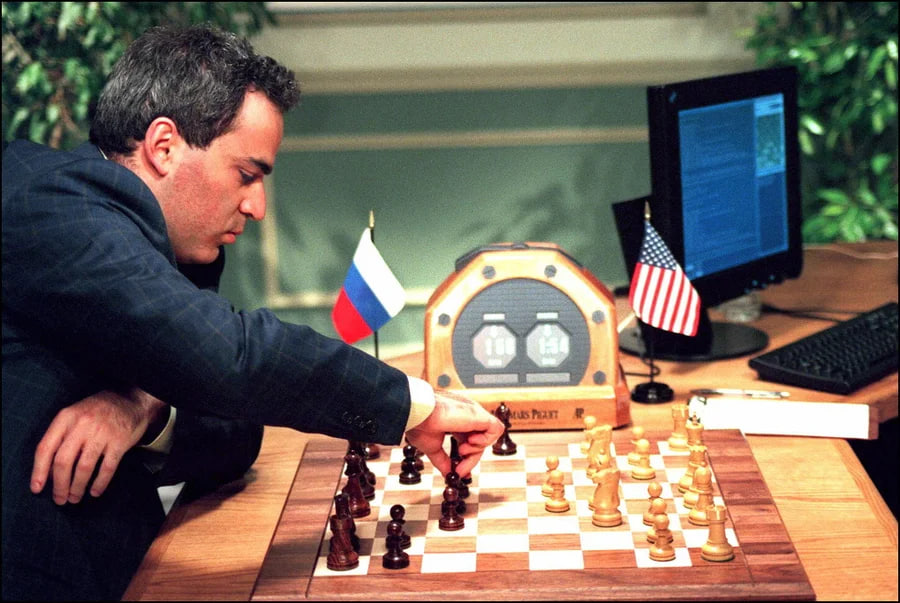
\includegraphics[width=0.6\textwidth]{assets/deepbluevskasparov.jpg}
    \caption{El campeón mundial de ajedrez Garry Kasparov (izq.) realiza un movimiento durante su cuarta partida contra \emph{Deep Blue}.}
    \label{fig:deepbluevskasparov}
\end{figure}


El hecho generó titulares en todo el mundo y 
revalorizó la supercomputación como herramienta de investigación 
científica. Medios como \emph{Scientific American} analizaron las 
implicaciones del triunfo, señalando cómo el empleo de 480 chips 
VLSI y 30 nodos RS/6000 SP redefinió las expectativas sobre el 
rendimiento de las máquinas \cite{greenemeier2017}. La repercusión 
académica fue inmediata: Carnegie Mellon otorgó el Premio Fredkin, 
valorado en 100 000 USD, y se multiplicaron los congresos y 
talleres dedicados a la paralelización extrema y al diseño de 
aceleradores especializados \cite{ibmHistoryDeepBlue}.

\subsection{Influencias posteriores}

Tras el éxito de \textit{Deep Blue}, el paradigma de desplazar 
cargas críticas de cálculo a hardware dedicado se expandió 
rápidamente. En el ámbito financiero, los \emph{hedge funds}\footnote{Fondos de inversión que utilizan una variedad de estrategias complejas para generar rendimientos, a menudo involucrando un alto grado de apalancamiento y riesgo.} 
adoptaron técnicas de \emph{cluster computing}\footnote{Conjunto de métodos y tecnologías utilizadas para coordinar y gestionar los recursos de un cluster de computadoras, optimizando el rendimiento y la eficiencia.} 
para simulaciones de 
riesgo en tiempo real, inspiradas en la arquitectura 
maestro-trabajador-chip de IBM \cite{aung2010}. Asimismo, la práctica 
de \emph{offloading} a 
aceleradores (ahora GPUs y FPGAs\footnote{GPUs (\emph{Graphics Processing Units}) son procesadores diseñados para el procesamiento paralelo de datos, especialmente imágenes. FPGAs (\emph{Field-Programmable Gate Arrays}) son circuitos integrados que pueden ser reprogramados después de su fabricación, lo que permite una gran flexibilidad en el diseño de hardware.}) 
se consolidó en aplicaciones de 
aprendizaje profundo, siguiendo el modelo pionero de \textit{Deep 
Blue} \cite{forbes2019explainable}.

\subsection{Repercusiones histórico-culturales}

El enfrentamiento humano-máquina suscitó reflexiones en filosofía y 
sociología de la ciencia sobre la confianza en sistemas automatizados. 
Documentales como \emph{Game Over: Kasparov and the Machine} (2003) 
examinaron las acusaciones de falta de transparencia en el diseño de 
\textit{Deep Blue}, alimentando la demanda de auditorías de “caja 
blanca” en sistemas críticos\footnote{Evaluación exhaustiva de un sistema, donde el auditor tiene acceso completo al código fuente, la documentación y la arquitectura del sistema, lo que permite una revisión detallada de la seguridad y la funcionalidad.}. 
A largo plazo, 
esta preocupación influyó en la creación de estándares de 
explicabilidad en IA, que hoy exigen trazabilidad de decisiones 
algorítmicas en sectores como la sanidad y la justicia 
\cite{korf1997does,bory2019deep}.

\subsection{Curiosidades}

Durante la cuarta partida de 1997, \textit{Deep Blue} ejecutó un 
movimiento inesperado (que Kasparov calificó de “creatividad” 
ante lo insólito), el cual años después se atribuyó a un desajuste 
en los parámetros de evaluación, no a un cálculo “creativo” de la 
máquina \cite{latson2015}. Este incidente ilustró la delgada línea 
entre la aparente originalidad de una IA y la complejidad de sus 
reglas internas, subrayando la importancia de la transparencia para 
comprender sus decisiones.

\section{Biografías}

\subsection*{Murray Campbell}

Murray S. Campbell (nacido en 1957 en Edmonton, Canadá) es un 
informático pionero en el campo del ajedrez computacional. 
Obtuvo su B.Sc.\ en Ciencias de la Computación en 1979 y su M.Sc.\ 
en 1981 en la University of Alberta, trabajando allí con Hans 
Berliner en el proyecto HiTech, campeón de la North American 
Computer Chess Championship en 1985 y 1989. 
En 1987 completó su Ph.D.\ en la Carnegie Mellon University con 
una tesis sobre la paralelización de la búsqueda alfa-beta en 
ajedrez, sentando las bases de sistemas como \emph{Deep Thought} 
\cite{icore2004bod}.

En 1989 se incorporó al IBM T.J.\ Watson Research Center, donde 
fue miembro clave del equipo que diseñó y construyó \emph{Deep Blue}, el 
primer ordenador en derrotar a un campeón mundial de ajedrez bajo 
condiciones de torneo en 1997. Campbell 
desarrolló principalmente la función de evaluación del sistema y 
colaboró estrechamente con el Gran Maestro Joel Benjamin en la 
preparación del libro de aperturas \cite{chessprog_murray}. 
Actualmente es Distinguished Research Scientist en el grupo AI 
Foundations de IBM, centrado en arquitecturas neuro-simbólicas y 
evaluación de capacidades de los sistemas de IA \cite{ibmCampbellBio}.


\subsection*{Feng-hsiung Hsu}

Feng-hsiung Hsu (nacido el 1 de enero de 1959 en Keelung, 
Taiwán) es un pionero taiwanés-estadounidense en ciencia de la 
computación e ingeniería eléctrica, célebre por diseñar los chips 
VLSI que impulsaron los sistemas \emph{ChipTest} y \emph{Deep Thought}, 
precursores directos de \textit{Deep Blue} 
\cite{chessprog_hsu}. Tras obtener su B.S.\ en 
Ingeniería Eléctrica en la Universidad Nacional de Taiwán, Hsu 
llegó a la Carnegie Mellon University en 1985 para cursar estudios 
de posgrado en computación, donde en 1989 defendió su tesis 
doctoral sobre la paralelización a gran escala de la búsqueda alfa-beta 
en ajedrez. Su trabajo durante ese período 
condujo al desarrollo de \emph{Deep Thought}, el primer programa en 
derrotar a un Gran Maestro en torneo oficial, y cimentó su rol 
como arquitecto principal del equipo IBM que, en 1997, consiguió 
que \textit{Deep Blue} venciera al campeón mundial Garry Kasparov 
\cite{ibmHistoryDeepBlue}.

Tras la gesta de 1997, Hsu amplió su carrera en la industria: en 
1997 se incorporó a Compaq/HP y, desde 2003, forma parte de 
Microsoft Research Asia en Pekín, donde ha continuado explorando 
arquitecturas paralelas y aplicaciones de inteligencia artificial. 
Entre sus reconocimientos destacan el ACM 
Grace Murray Hopper Award de 1991 y el IEEE Mephisto 
Best-Publication Award, además de ser autor de \emph{Behind Deep 
Blue: Building the Computer that Defeated the World Chess Champion} 
(Princeton University Press, 2002), obra de referencia sobre la 
historia y la ingeniería de \textit{Deep Blue} \cite{hsu2022behind}. 
Su legado perdura en la adopción de aceleradores de hardware y 
diseños híbridos en múltiples dominios científicos y empresariales.

\subsection*{A. Joseph “Joe” Hoane Jr.}

A. Joseph Hoane Jr. (nacido en 1962) es un científico de la 
computación y ingeniero de software estadounidense, reconocido por 
su papel como ingeniero de software principal en el proyecto 
\emph{Deep Blue}. Tras obtener su licenciatura en Ciencias de la 
Computación por la Universidad de Illinois en Urbana-Champaign en 
1984 y un máster en la misma especialidad en Columbia University 
en 1994, Hoane se incorporó a IBM Research en noviembre de 1990 
para unirse al equipo entonces denominado \emph{Deep Thought}, 
que más 
tarde sería renombrado \emph{Deep Blue} \cite{chessprog_hoane}.  

Como responsable del desarrollo del algoritmo de búsqueda 
paralela, Hoane diseñó y optimizó la coordinación entre el clúster 
RS/6000 SP y los chips VLSI especializados, asegurando un balance 
de carga eficiente y una escalabilidad que culminó en la victoria 
histórica contra Garry Kasparov \cite{ibmHistoryDeepBlue}. 
Además de sus contribuciones en \emph{Deep Blue}, ha coautoreado artículos 
fundamentales como “\emph{Deep Blue} System Overview” (1995) \cite{hsu1995deep} y 
“Search Control Methods in \emph{Deep Blue}” (1999) \cite{campbell1999search}, 
que documentan las 
innovaciones de software que permitieron combinar de manera 
efectiva técnicas de búsqueda selectiva con la gran capacidad de 
procesamiento en silicio.

\subsection*{Thomas S. Anantharaman}

Thomas S. Anantharaman nació en 1962 en Varanasi, India. 
Obtuvo su B.Tech en Ingeniería Electrónica en 1982 por el 
Institute of Technology, Banaras Hindu University, habiendo 
logrado el segundo puesto en el examen de ingreso IIT-JEE de 1977 
\cite{itbhu_anantharaman}. Posteriormente se trasladó a la 
Carnegie Mellon University, donde entre 1985 y 1990 colaboró con 
Feng-hsiung Hsu y Murray Campbell en los proyectos \emph{ChipTest} y 
\emph{Deep Thought}. Su investigación culminó con la defensa de la tesis 
doctoral “A Statistical Study of Selective Min-Max Search in 
Computer Chess” en 1990 \cite{anantharaman1990statistical}, trabajo que sentó las bases algorítmicas 
para \emph{Deep Blue} \cite{chessprog_anantharaman}.

Tras completar su doctorado, Anantharaman orientó su carrera hacia 
la bioinformática, especializándose en métodos bayesianos para el 
análisis de tecnologías de mapeo óptico de moléculas. En la 
actualidad ejerce como Senior Bioinformatics Software Engineer en 
BioNano Genomics, en San Diego, donde lidera el desarrollo de 
software para el ensamblaje y análisis de mapas genómicos de 
moléculas individuales \cite{linkedin_anantharaman}.  

\subsection*{Andreas G. Nowatzyk}

Andreas G. Nowatzyk nació en Alemania y obtuvo titulaciones en 
Física y en Ciencias de la Computación en la Universität Hamburg, 
Alemania. Posteriormente cursó el doctorado en Ciencias de la 
Computación en Carnegie Mellon University, donde se graduó en 1989 
tras investigar sistemas de comunicación de alta velocidad y 
multiprocesamiento \cite{cmuNowatzyk}. Durante sus años de 
posgrado contribuyó al diseño de la arquitectura y la coherencia 
de caché en el proyecto S3.mp de Sun Microsystems, liderando 
investigaciones sobre modelos de memoria compartida escalable 
\cite{s3mpNowatzyk}.

Entre 1987 y 1990 formó parte del equipo \emph{Deep Thought} en Carnegie 
Mellon, colaborando en el afinamiento de la función de evaluación \cite{chessprogNowatzyk}. 
Tras su paso por 
\emph{Deep Thought}, Nowatzyk trabajó en Digital Equipment Corporation y 
en los laboratorios de Compaq, especializándose en arquitecturas 
heterogéneas de multiprocesamiento y, más recientemente, ocupa el 
puesto de Principal Investigator en Google, donde investiga 
aceleradores hardware y sistemas paralelos de alta eficiencia 
\cite{cmuNowatzyk}.


\subsection*{Michael “Mike” Browne}

Michael “Mike” Browne es un ingeniero de software e investigador 
que formó parte del equipo original de \emph{Deep Thought} en 
Carnegie Mellon, precursor directo de \emph{Deep Blue}. En la fase 
inicial (1987-1989), Browne colaboró con Feng-hsiung Hsu, Thomas 
Anantharaman y Murray Campbell en el diseño e implementación del 
generador de movimientos y de los módulos de evaluación heurística 
de los chips VLSI, contribuyendo a que \emph{Deep Thought} se convirtiera 
en la primera máquina en derrotar a un gran maestro en torneo 
oficial \cite{chessprog_deepthought}. Tras la adquisición del 
proyecto por IBM y su evolución hasta \emph{Deep Blue}, Browne continuó 
apoyando la integración de software y hardware especializados que 
culminó en la histórica victoria frente a Garry Kasparov 
\cite{ibmHistoryDeepBlue}.



\begin{figure}[h]
    \centering
    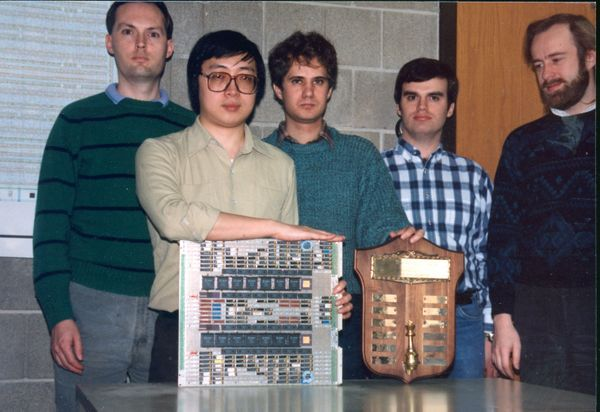
\includegraphics[width=0.6\textwidth]{assets/team.jpg}
    \caption{Murray Campbell, Feng-hsiung Hsu, Thomas Anantharaman, Mike Browne y Andreas Nowatzyk
    después de ganar el Premio Fredkin por el desempeño a nivel de Gran Maestro de \emph{Deep Thought}.}
    \label{fig:team2}
\end{figure}



\newpage
% region Conclusiones
% Conclusiones
\section{Conclusiones}


La experiencia de \textit{Deep Blue} pone de manifiesto cómo la 
confluencia de tres líneas de innovación (\emph{hardware} VLSI 
especializado, algoritmos de búsqueda selectiva y bases de datos 
inteligentes) permitió superar las barreras históricas entre el 
ajedrez humano y la computadora. En primer lugar, los chips 
VLSI diseñados \emph{ad hoc}\footnote{Chips diseñados para un propósito específico y no para uso general. Este diseño personalizado permite optimizar el rendimiento para la tarea deseada.} 
para generación de movimientos y 
evaluación en un ciclo de reloj demostraron que el procesamiento 
masivamente paralelo podía explotar la fuerza bruta sin 
sacrificar precisión táctica \cite{campbell2002deep}. 
En segundo lugar, el algoritmo de “\emph{dual credit with delayed 
extensions}” introdujo una búsqueda altamente no uniforme que 
adaptaba dinámicamente la profundidad según la complejidad de 
la posición, con extensiones fraccionarias que prevenían 
explosiones combinatorias y preservaban robustez frente a 
amenazas tácticas \cite{aung2010}. Por último, la 
integración de un libro principal, un “\emph{extended book}” de 700 000 
partidas y bases de finales con todos los casos de hasta cinco 
piezas (y casos seleccionados de seis piezas) proporcionó un conocimiento posicional sólido que 
complementó el poder de cómputo, reduciendo la dependencia en 
el cálculo exhaustivo en fases teóricamente bien entendidas 
\cite{greenemeier2017}.

Históricamente, la victoria de \textit{Deep Blue} sobre Garry 
Kasparov en 1997 simboliza el tránsito de la IA simbólica y de 
fuerza bruta hacia sistemas híbridos que combinan aprendizaje 
experto con arquitecturas de alto rendimiento. 
Este hito no sólo impulsó la investigación en supercomputación y 
en aceleradores especializados (preludiando el uso extensivo de 
GPUs y FPGAs en IA), sino que también abrió el camino para metodologías 
que hoy sustentan desde la biología computacional hasta el 
análisis financiero en tiempo real \cite{wired2017ai}. 
En suma, \textit{Deep Blue} demostró que el equilibrio entre 
conocimiento experto, paralelismo extremo y algoritmos 
selectivos puede superar la fuerza bruta pura, marcando el 
umbral de la era moderna de la inteligencia artificial aplicada.



\newpage
% region Bibliografía
% Bibliografía
\bibliography{build/referencias}



\end{document}